\documentclass[12 pt]{article}
\hbadness=10


\usepackage{amsmath, amssymb, amsfonts, setspace, stmaryrd, amsthm, graphicx, tikz}

\usepackage[utf8]{inputenc}
\usepackage[english]{babel}
\usetikzlibrary{positioning}% To get more advanced positioning options
\usetikzlibrary{arrows}% To get more arrow heads
\usepackage{hyperref} % Allows to make references and links clickable

\usepackage[margin=1.5in]{geometry}
\newtheorem{theorem}{Theorem}
\newtheorem{definition}{Definition}
%%align* environment
\newcommand{\eq}[1]{\begin{align*}#1\end{align*}}

%Math commands
\DeclareMathOperator{\R}{\mathbb{R}}
\DeclareMathOperator{\C}{\mathbb{C}}
\DeclareMathOperator{\Z}{\mathbb{Z}}
\DeclareMathOperator{\N}{\mathbb{N}}
\DeclareMathOperator{\Q}{\mathbb{Q}}

%%%% added by NG
\usetikzlibrary{shapes,backgrounds,decorations,patterns}
\usepackage{pgfplots}
% externalize the figures
% \usepgfplotslibrary{external
% \tikzexternalize

%Crypto commands
\usepackage{cryptocode}
\newcommand{\sample}{\hskip2.3pt{\gets\!\!\mbox{\tiny${\$}$\normalsize}}\,}
\def\D{\ensuremath{\mathcal{D}}}
\def\A{\ensuremath{\mathcal{A}}}
\def\ss{\ensuremath{\mathcal{S}}}
\def\bin{\ensuremath{\{0, 1\}}}

%comments
\newcommand{\nsm}[1]{\textcolor{teal}{(NG: #1)}}
\newcommand{\new}[1]{\textcolor{blue}{#1}}
\newcommand{\todo}[1]{\textcolor{red}{#1}}

\renewcommand\abstractname{Introduction}

\newcounter{exercise}[section]
\newenvironment{exercise}{\refstepcounter{exercise}\par\bigskip \begin{quotation}{}{\leftmargin .25in\rightmargin .25in}
    \noindent \textbf{Exercise~\thesection.\theexercise }  \rmfamily}{\end{quotation}\par\bigskip}
\newcommand{\exref}[1]{\hyperref[#1]{\thesection.\ref*{#1}}}

\newenvironment{bonus}{\refstepcounter{exercise}\par\bigskip \begin{quotation}{}{\leftmargin .25in\rightmargin .25in}
    \noindent \textbf{*Bonus Exercise*~\thesection.\theexercise }  \rmfamily}{\end{quotation}\par\bigskip}

\newcounter{example}[section]
\newenvironment{example}{\refstepcounter{example}\par\bigskip \begin{quotation}{}{\leftmargin .25in\rightmargin .25in}
    \noindent \textbf{Example~\thesection.\theexample }  \rmfamily}{\end{quotation}\par\bigskip}

\title{Cryptographic Secret Sharing}
\author{Girls Talk Math}
\date{}

\begin{document}
% \color{blue}
\maketitle
\vskip 1in
\begin{center} \textbf{Introduction} \end{center}

\indent In this problem set, you will learn how to use math to split secrets into pieces. This is the cryptographic technique known as secret sharing and is the basis for many useful tools being deployed by companies today.

One last note about reading mathematical texts: it is very normal when reading math to read a passage or even a single sentence several times before understanding it properly. Also, never trust the author! Check every claim and calculation (time permitting). Take your time and never give up. Let's talk math!

\newpage

\tableofcontents
\vspace*{\fill}
Optional sections are marked with an asterisk (*).

%%%%%%%%%%%%%%%%%%%%%%
%%% Use \section{}, \subsection{}, etc. for different parts of the problem set. Start a newpage for a new section
%%%%%%%%%%%%%%%%%%%%%%

%%%%%%%%%%%%%%%%%%%%%%%%%%%%%%%%%
%%%
%%% Embed exercises in section as appropriate 
%%% 
%%%%%%%%%%%%%%%%%%%%%%%%%%%%%%%%%%%

\newpage


\section{Probability and Randomness}\label{sec:prob}

In mathematics, the word ``random'' has a more precise meaning that in everyday 
speech. Something is random if its outcome is governed by some \emph{probability 
distribution}. For example, the outcome $c$ of a coin toss is not fixed, but takes 
on one of the values in the set $\{H, T\}$, where $H$ means heads and $T$ means 
tails. (This is called the \emph{sample space} of $c$.) We write 
that $c \in \{H,T\}$, where the symbol $\in$ is read aloud as 
``is an element of'' or simply ``is in''.
The value of $c$ is described by the distribution $\left\{\frac{1}{2}, 
\frac{1}{2}\right\}$, which says that each outcome happens with 
probability one-half.

A variable like $c$ that represents an outcome or event is called a \emph{random 
variable}, since it can take on one of several values based on an underlying 
probability distribution. A random variable is \emph{uniformly random} if every possible 
value is equally likely. In other words, its probability distribution is the 
\emph{uniform distribution}. The variable $c$ is uniformly random (or simply \emph{uniform}).

\begin{exercise}
    Write ``uniform'' or ``not uniform'' for each of the following random variables:
    \renewcommand{\labelenumi}{(\alph{enumi})} 
    \begin{enumerate}
        \item Drawing a card from a shuffled deck.
        \item Drawing a card from an ordered deck.
        \item The weather on a given day.
        \item The outcome of a dice roll.
        \item The birthday of the first person you encounter on the street.
    \end{enumerate}
\end{exercise}

When a random variable is uniform, we say it is chosen \emph{uniformly at random} 
(sometimes shortened to chosen \emph{uniformly}) and denote this with the symbol 
$\sample$. For example, the outcome $c$ of a coin toss can be written as $c \sample 
\{H, T\}$ to mean that $c$ is sampled uniformly from the set $\{H, T\}$. 
% \nsm{Link to an external resource instead of explaining everything.}
\nsm{I use the notation $\sample$ because it is widespread in cryptography. 
$c \sample S$ has a slightly different meaning than $U(S)$, since it 
concerns itself with the \emph{variable} $c$ instead of representing 
a distribution.}

\begin{exercise}
    How would you represent a dice roll using the $\sample$ notation?
\end{exercise}

We use $\Pr$ to denote the probability of some event. For instance, the 
probability that $c$ is heads is one-half. In mathematical notation this
is written as
\[
    \Pr[c=H] = \frac{1}{2}
\]
Similarly, $c$ is tails with probability one-half:
\[
    \Pr[c=T] = \frac{1}{2}
\]

\new{Given these two facts, what is the probability of getting heads \emph{or}
tails? Because these two events are \emph{mutually exclusive} (that is, 
if one occurs, it means the other cannot possibly have occured, and 
vice versa), we can add their probabilities:}
\begin{align*}
    \Pr[c = H \text{ or } T] &= \Pr[c=H] + \Pr[c=T] \\
    &= \frac{1}{2} + \frac{1}{2} = 1
\end{align*}

Notice that these probabilities sum to 1. 
This is a common requirement of all probability distributions: the sum of their 
probabilities must be 1. This is the same as saying that \emph{one of} the possible events 
in the distribution happens with 100\% probability. If the sum was less than 1, it 
would mean that there's some other event that could happen instead, so the distribution
is incomplete. % If it was greater than 1, then the 

The pie charts below illustrate this idea. On the left is the probability 
distribution of a coin toss; on the right, the probability distribution 
of a dice roll. Notice that in both cases, the probabilities sum to 1.

\begin{figure}[h]
    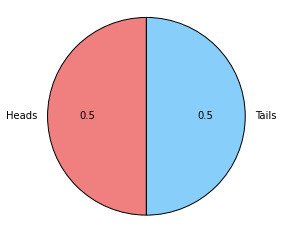
\includegraphics[width=.5\linewidth]{coin-pie.png}
    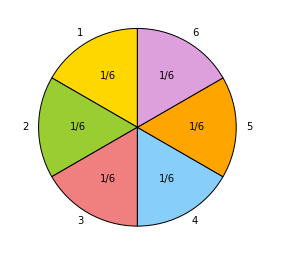
\includegraphics[width=.5\linewidth]{die-pie.png}
    % \caption{Left: probability distribution of a coin toss. Right: 
    % probability distribution of a dice roll. Probabilities always 
    % sum to 1.}
    \label{fig:pies}
  \end{figure}

\new{When two events are not mutually exclusive, however, we can't add 
their probabilities. For example, what's the probability of rolling a 
multiple of 2 or a multiple of 3? These are not mutually exclusive
events, since 6 is a multiple of \emph{both} 2 and 3! Instead, we need 
to break this question into mutually exclusive events. For example, we 
could consider the probability of rolling a multiple of two, and add 
this to the probability of rolling a 3: by doing this, we still cover 
all the possible outcomes (2, 3, 4, and 6) but broken into mutually 
exclusive events ($\{2,4,6\}$ or $\{3\}$) instead of overlapping events 
($\{2, 4, 6\}$ or $\{3, 6\}$). Then}

\begin{align*}
    &\Pr[d \text{ is a multiple of 2 or 3}] \\
    &= \Pr[d \text{ is even}] + \Pr[d=3]\\
    &= \frac{1}{2} + \frac{1}{6}\\
    &= \frac{4}{6} = \frac{2}{3}
\end{align*}

\new{where $d$ is the random variable representing the outcome of the die roll.}

\hfill\\
\nsm{Moved conditional probability before independence.}

Conditional probability is the probability that something occurs 
provided that another event occurred. This is written with the symbol 
$\mid$, which is read aloud as ``given''. So, $\Pr[A \mid B]$ is 
read as ``the probability of $A$ given $B$''.

For example, it's more likely to be raining if the sky is cloudy 
than if it's clear. We can write this as
\[
    \Pr[\text{raining} \mid \text{cloudy sky}] >
    \Pr[\text{raining} \mid \text{clear sky}]
\]

The following equality about conditional probability always holds:
\begin{subequations}\label{eq:conditional}
    \begin{equation}
        \Pr[A \mid B] = \frac{\Pr[A \text{ and } B]}{\Pr[B]}
        \label{eqn:conditional_mid}
    \end{equation}
An alternate form is
    \begin{equation}
        \Pr[A \text{ and } B] = \Pr[A \mid B] \cdot \Pr[B]
        \label{eqn:conditional_and}
    \end{equation}
\end{subequations}

\nsm{I'm not sure if the explanation that follows is beneficial.}
\new{Understanding why these equations are true can help us remember them.
One way to see why they hold is with a Venn diagram:}

\begin{center}
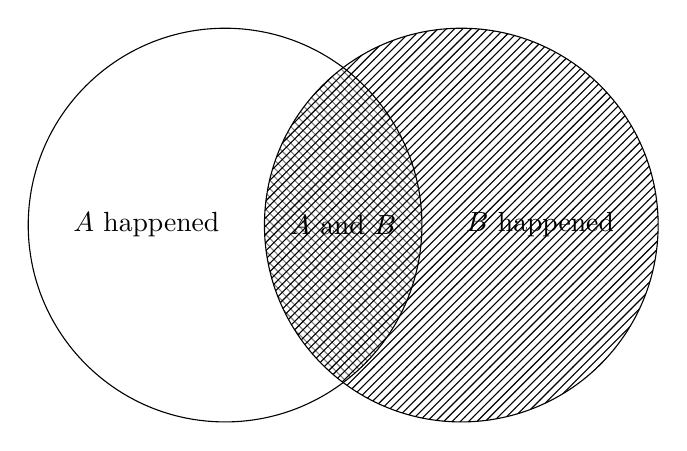
\begin{tikzpicture}
    % A
    \node[draw,%anchor=west,
        circle,minimum size=5cm,
        % label={0:$A$},
        ]                           (A) at (0,0) {};
    % B
    \node[draw,%anchor=east,
        pattern=north east lines,
        fill opacity=0.5,
        circle,minimum size=5cm,
        % label={45:$B$},
        ]                           (B) at (3,0) {};
    % labels
    \node                               at (1.5,0) {$A$ and $B$};
    \node                               at (-1,0) {$A$ happened};
    \node                               at (4,0) {$B$ happened};

    \begin{scope}
        \clip (0,0) circle(2.5cm);
        \clip (3,0) circle(2.5cm);
        \fill[pattern=north west lines,
            opacity=0.5
            ]                       (0,0) circle(2.5cm);
    \end{scope}
\end{tikzpicture}
\end{center}

\new{Let's think through Equation~\ref{eqn:conditional_mid} with this diagram 
in front of us. The event ``$A$ given $B$'' means we know $B$ happened, 
so now our entire realm of possibilities exists only in the circle 
on the right. Let's zoom in on that circle:} 

\begin{center}
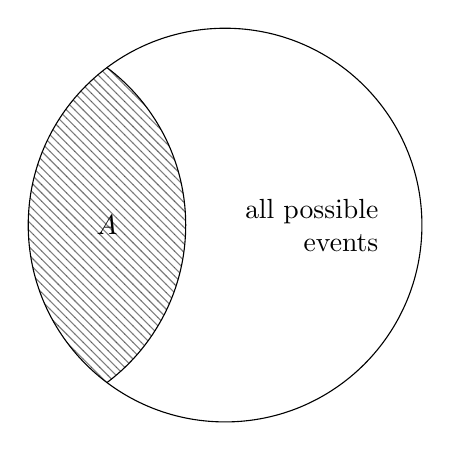
\begin{tikzpicture}
    % B
    \node[draw,%anchor=east,
        circle,minimum size=5cm,
        % label={45:$B$},
        ]                           (B) at (0,0) {};
    % labels
    \node[align=right]                        at (1.1,0) {all possible\\events};
    \node                                     at (-1.5,0) {$A$};

    \begin{scope}
        \clip (0,0) circle(2.5cm);
        \draw (-3,0) circle(2.5cm);
    \end{scope}
    \begin{scope}
        \clip (0,0) circle(2.5cm);
        \clip (-3,0) circle(2.5cm);
        \fill[pattern=north west lines,
            opacity=0.5
            ]                       (0,0) circle(2.5cm);
    \end{scope}
\end{tikzpicture}
\end{center}
\new{The cases in which $A$ happens next are in the little slice on the 
left. We want to know the probability $A$ happening given our current 
information, which is simply the fraction of possible events covered by 
this area. Zooming back out, that's exactly $\Pr[A \text{ and } B]$ 
divided by $\Pr[B]$!}

\new{The difference is the reference frame: in the first diagram, we are in a 
world in which we make no assumptions: all possibilities are open. In 
the second, we are using the extra information that $B$ happened to 
limit the world of possibilities. Let's see a concrete example next.}

\begin{example}
\nsm{Thanks, Seyed, for suggesting this example!}
    Suppose your friend rolls a die without showing you the result.
    You know the probability that they rolled a 3 is $\frac{1}{6}$. Now 
    suppose they tell you, ``I rolled an odd number.'' Using this additional 
    information, you can update your estimate of the probability that the 
    die roll is a 3 to $\frac{1}{3}$, since you know the die landed with 
    equal probability on 1, 3, or 5, and definitely didn't land on 2, 4, 
    or 6.

    Written in the language of conditional probability, this is
    \begin{align*}
        \Pr[d = 3 \mid d \text{ is odd}] 
        &= \frac{
                \Pr[d=3 \text{ and } d \text{ is odd}]
            }{
                \Pr[d \text{ is odd}]
            }\\
        &= \frac{
                \Pr[d=3]
            }{
                \Pr[d \text{ is odd}]
            }\\
        &= \frac{1}{6} \div \frac{1}{2} = \frac{2}{6} = \frac{1}{3}
    \end{align*}
\end{example}

In some cases, we have $\Pr[A \mid B]=\Pr[A]$. Intuitively, this means 
that the probability of $A$ is the same regardless or whether or not $B$
happened. For example, a good coin toss should be independent of the coin 
used for the toss or the person doing the toss.
In these cases, we say that $A$ and $B$ are \emph{independent} events, and 
their corresponding random variables are independent. Then Equation~\ref{eqn:conditional_and}
simplifies to 
\[
   \Pr[A \text{ and } B] = \Pr[A] \cdot \Pr[B]
\]. 
This means that for independet random variables, we can just multiply the probabilities 
of two events together to get the probability that both events happen simultaneously.

\begin{example}
    Suppose I roll a die and flip a coin. What's the probability that I roll a 1 
    \emph{and} get heads?

    The dice and coin outcomes are independent, so we can multiply the probabilities
    of the two events together the get the probability of both events occuring. Let 
    $d$ be the random variable representing the outcome of the die roll and $c$ 
    be the random variable representing the outcome of the coin toss. Then 

    \begin{align*}
        &\Pr[d=1 \text{ and } c=H]\\
        =& \Pr[d=1] \cdot \Pr[c=H]\\
        =& \frac{1}{6} \cdot \frac{1}{2} = \frac{1}{12}
    \end{align*}
\end{example}

\begin{exercise}
    Suppose I flip two coins. What's the probability of both coins landing on heads?
\end{exercise}

Let's put everything we've learned so far together and work through some examples. 
Remember, for the \textbf{or} of two mutually exclusive events, we add; 
for the \textbf{and} of two independent events, we multiply. In the latter 
case, if the events aren't mutually exclusive, we use conditional probability 
(Equations~\ref{eqn:conditional_mid} and~\ref{eqn:conditional_and}).

\begin{example}
    Say I flip a fair coin twice. What's the probability of getting the 
    same result both times?

    There are two ways of getting the same result on both flips: we either 
    get heads twice (HH) or tails twice (TT):
    \[
        \Pr[HH] + \Pr[TT]
    \]

    Because subsequent coin flips are independent of each other, this is equal to 
    \[
        \Pr[H]\cdot \Pr[H] + \Pr[T]\cdot\Pr[T]
    \]

    Since the coin is fair, each outcome (heads or tails) happens with equal 
    probability, so this equals
    \begin{align*}
        & \frac{1}{2}\cdot\frac{1}{2} + 
        \frac{1}{2}\cdot\frac{1}{2}\\
        =& \frac{1}{4} + \frac{1}{4}\\
        =& \frac{1}{2}
    \end{align*}
\end{example}

\begin{exercise}
    Suppose I only flip a coin again if my first coin toss came out tails. 
    What's the probability of getting one heads outcome?
\end{exercise}

\begin{exercise} The following questions deal with rolling a 6-sided die.
    \renewcommand{\labelenumi}{(\alph{enumi})} 
    \begin{enumerate}
        \item What's the probability of rolling an even number?
        \item What's the probability of rolling a 1 followed immediately by a 2?
        \item If I roll twice, what's the probability that my second roll will 
        be higher than my first?
        \item Suppose that when I roll a 1, I get to reroll and use the 
        second number instead. What's the probability of rolling a 5 or higher?
    \end{enumerate}
\end{exercise}

When two random variables have the same underlying probability 
distribution, we say they are \emph{indistinguishable}. For example,
if $c \in \{HHH, HHT,\allowbreak HTH, HTT, THH, THT, TTH, TTT\}$ 
is the random variable representing the outcome of three coin tosses,
the probability distribution of $c$ is 
\begin{align*}
    \left\{
        \frac{1}{8},\frac{1}{8},\frac{1}{8},\frac{1}{8},
        \frac{1}{8},\frac{1}{8},\frac{1}{8},\frac{1}{8}
    \right\}
\end{align*}

where each probability is the probability that $c$ takes on the 
corresponding value in the sample space.

Compare this to the probability distribution of the random 
variable $d \in \{1,2,3,4,5,6,7,8\}$ for rolling an 8-sided die:
\[
    \left\{
        \frac{1}{8},\frac{1}{8},\frac{1}{8},\frac{1}{8},
        \frac{1}{8},\frac{1}{8},\frac{1}{8},\frac{1}{8}
    \right\}
\]

They're the same distribution! Therefore $c$ and $d$ are 
indistinguishable.

\begin{exercise}
    Write ``indistinguishable'' or ``not indistinguishable''
    for each pair of probability distributions $D_1, D_2$:
    \renewcommand{\labelenumi}{(\alph{enumi})} 
    \begin{enumerate}
        \item $D_1$: Rolling an even or an odd number on a 6-sided die, 
        $D_2$: getting heads or tails when you flip a coin
        \item $D_1$: Drawing a random card from a deck, $D_2$: rolling a 6-sided 
        die and flipping 3 coins
        \item $D_1$: Whether or not you get at least one heads when flipping
        two coins, $D_2$: whether or not you draw a club from a shuffled 
        deck.
    \end{enumerate}
\end{exercise}

\subsection{Randomness in Cryptography}

As we'll see, randomness plays an extremely important role in modern cryptographic
schemes. A cryptographic \emph{scheme} is a well-defined procedure for accomplishing 
some goal (called a \emph{cryptographic primitive}). For example, the Caesar 
cipher is an encryption scheme, meaning it is a procedure for accomplishing
the cryptographic primitive of encryption. 
In this packet, you'll learn about several \emph{secret sharing} schemes.

When a scheme's security rests only on the randomness used in it, and not on 
solving a difficult or very long problem, we say that scheme is
\emph{information-theoretically secure}. This is different from, for example,
the schemes in the RSA cryptography packet, whose security depends on 
the assumed difficulty factoring\footnotemark.

\footnotetext{When a scheme is protected by how hard it is 
to compute something, it is said to be \emph{computationally secure}.}

The exact level of security of a scheme is determined by a \emph{security 
parameter}, which is a number that's often denoted by the symbol $\lambda$ 
(the Greek letter lambda). The people using a scheme will generally decide 
on the security parameter ahead of time based on how secure they want to 
be. There's usually a tradeoff between security and efficiency, so the 
parties will settle on a $\lambda$ that makes them feel safe enough without 
making their computations prohibitively slow (hours, days, or weeks).
% We'll learn more about this in Section~\ref{sec:proof}.
% TODO: future version could have an example where lambda is too small 
% and show that an adversary can guess $s_1$ with non-negligible probability.

Lambda is usually set to a large power of two, like 128 or 256; to keep 
numbers reasonable in this packet, though, we'll let $\lambda=10$.

\newpage
\section{Secret Sharing}\label{sec:ss}
\emph{Secret sharing} is a way to ``split'' a secret value (call it $s$ for 
``secret'') into pieces, called \emph{shares}. 
Two useful properties a secret sharing scheme might have are \emph{correctness} and 
\emph{privacy}. Informally, correctness means that if we put shares back together, 
we get back the original secret; privacy says that each share by itself reveals 
nothing about the secret $s$. 

These properties are important for practical uses of secret sharing. For 
example, using secret sharing, we can distribute shares among a large set of people so that no one 
knows the secret but some subset of them can recover the secret if they 
pool their information.

We'll be a little more rigorous about these definitions soon, but first, let's 
see an example.  

\subsection{A simple secret sharing}

Here is a simple scheme for sharing integers using nothing but addition and subtraction:

\def\share{\ensuremath{\mathsf{Share}}}
\def\rec{\ensuremath{\mathsf{Rec}}}

\begin{figure}[h!]
\begin{pchstack}[center]
\fbox{%
\procedure{$\share(s)$}{%
    s_1 \sample \{1, \ldots, 2^\lambda\} \\
    \pcreturn (s_1, s - s_1)
}
\pchspace
\procedure{$\rec(s_1, s_2)$}{%
    \pcreturn s_1 + s_2
}
}
\end{pchstack}
\caption{Additive secret sharing scheme}
\label{fig:additiveSS}
\end{figure}

Let's go through the notation together. First, on the left, we see that 
the $\share$ algorithm is being defined. (An \emph{algorithm} is simply a procedure.)
The parentheses after the name tell us that it takes an input $s$, which in 
this context is the secret to be shared. The first line tells us to sample\footnotemark~
an element from the set $\{1, \ldots, 2^\lambda\}$ and call it $s_1$. The 
dots in the set are shorthand for all the numbers in between. For instance, 
when $\lambda=10$, we sample $s_1$ uniformly from the set $\{1, 2, 3, 4, \ldots, 
1022,1023, 1024\}$. Now we're almost done! The next line says to return 
(output) a pair of numbers: the random number $s_1$ and the difference $s-s_1$.
\footnotetext{We introduced the symbol $\sample$ in Section~\ref{sec:prob}.}

To summarize, $\share$ converts a secret $s$ into a two shares. Okay, so how can 
two people, each with one of the shares, get back the original secret? That's
what the right side of Figure~\ref{fig:additiveSS} tells us. The reconstruction 
algorithm $\rec$ takes two integers (call them $s_1$ and $s_2$) and returns their 
sum. That's it!

If $\rec$ receives two shares that were produced by the $\share$ algorithm, 
it will return $s_1 + (s-s_1) = s$. This means the scheme has correctness!
What about privacy? 

It turns out the scheme is private as well: someone who sees only one of the two 
shares learns nothing about the secret. This is pretty straightforward if the 
one share you see is $s_1$: we picked this value randomly (remember this means 
we picked it independently of $s$), so it has nothing to do with $s$. This 
is the case with the share $s-s_1$ as well. If we're given a number $s_2$ 
calculated as $s-s_1$, we don't know the other share $s_1$, so $s_2$ could 
be anything: $s-0$, $s-1$, $s-2$, and so on. Another way to think about this 
is that we don't know $s_1$, so we can't undo the subtraction and recover $s$.
In this case we say that $s_1$ ``masks'' $s$.

These arguments for correctness and privacy are not very rigorous. We'll 
take a look at how cryptographers prove these properties in Sections~\ref{sec:formal-defs} 
and \ref{sec:proof}.

\begin{exercise}
    Pick your favorite number and secret share it using the \share~algorithm 
    defined above, with $\lambda=10$. (Hint: $2^{10}=1024$.)
    (Repeat this exercise until you are comfortable with this secret sharing 
    scheme.)
\end{exercise}

\begin{exercise}
    What is
    \renewcommand{\labelenumi}{(\alph{enumi})} 
    \begin{enumerate}%[label={(\arabic*)}] %\usepackage{enumitem}
        \item $\rec(2, 6)$?
        \item $\rec(4, 1)$?
        \item $\rec(10, 2)$?
        \item $\rec(115, -103)$?
        \item $\rec(559, -544)$?
    \end{enumerate}
\end{exercise}

\begin{exercise}
    Can you adapt this additive secret sharing scheme to output 
    3 shares instead of 2? How does this change the reconstruction 
    algorithm?
\end{exercise}

\subsection{Formal Definitions*}\label{sec:formal-defs}

We'll now formally define what it means to be a secret sharing scheme and the 
properties such a scheme might have, using the standard notation in 
cryptography. First, we'll define what a secret sharing scheme 
does without giving implementation details (there could be multiple ways 
of achieving the same thing, after all). 

% This is the n-out-of-n definition
\begin{definition}[Secret sharing scheme]\label{def:ss}
    Let $\D$ be the input domain and $\D_s$ be the share domain.
    A secret sharing scheme is a pair of efficient algorithms $(\share, \rec)$
    and an associated natural number $n$ such that

    \begin{itemize}
        \item \share~takes as input a secret $s \in \D$ and outputs $n$ 
        shares in $\D_s$.
        \item \rec~takes as input $m$ shares $s_1, \ldots, s_m \in D_s$ 
        and output some value $y \in \D$ or a special symbol $\perp$ 
        indicating failure. (If $m \neq n$, it outputs $\perp$.)
    \end{itemize}
\end{definition}
% from Input Auth paper
% \begin{definition}[secret-sharing scheme]
%     A pair of polynomial-time algorithms $\Sigma = (\share, \recon)$ is a (two-party) secret-sharing scheme if
%     \begin{itemize}
%         \item $\share$ takes as input a security parameter $\secparam$ and a value $x$ in the domain $\mathcal{D}_\kappa$ associated with~$\kappa$ (e.g., $\mathcal{D}_\kappa = \bin^\kappa$) and outputs two shares $\sh_1, \sh_2$. We assume $\kappa$ is implicit in each share.
%         \item $\recon$ takes as input two shares and outputs either a value $y \in \mathcal{D}_\kappa$ or a distinguished symbol $\perp$.
%     \end{itemize}
%     For correctness, we require that for all $\kappa$ and $x \in \mathcal{D}_\kappa$, $\recon(\share(\secparam, x)) = x$.
% \end{definition}


Here's a visual representation: \nsm{Is this less confusing?}

\begin{center}
\pgfdeclarelayer{background}
\pgfsetlayers{background,main}
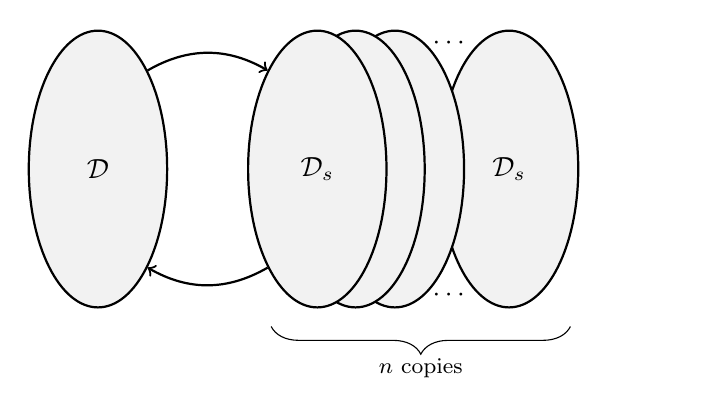
\begin{tikzpicture}[
    ovalnode/.style={ellipse, draw, fill=gray!10,align=center,minimum width=50pt, minimum height=100pt, thick},
]
    % Nodes
    \node[ovalnode] (domain)                         {$\D$};
    \node[ovalnode] (range1)  [right=of domain]      {$\D_s$};
    \begin{pgfonlayer}{background}
        \node[ovalnode] [right=of range1,xshift=-0.35cm] {$\D_s$};
        \node[text width=3cm]     at (5.75,1.6)              {$\cdots$};
        \node[text width=3cm]     at (5.75,-1.6)              {$\cdots$};
        \node[ovalnode] [right=of range1,xshift=-1.8cm] {};
        \node[ovalnode] [right=of range1,xshift=-2.3cm] {};
    \end{pgfonlayer}
    \draw [decorate,decoration={brace,amplitude=10pt,mirror},yshift=0pt]
    (2.2,-2) -- (6,-2) node [black,midway,yshift=-1.5em] 
    {\footnotesize $n$ copies};

    % \node[text width=3cm]     at (5.45,0)              {$\cdots$};
    % \node[ovalnode] (rangen)  [right=of range1]      {$\D_s$};

    % Lines
    \draw[thick,->] (domain.north east) to[out=30,in=150] 
    node[draw=none,fill=none,font=\small,midway,above] {$\share$}
    (range1.north west);
    \draw[thick,->] (range1.south west) to[out=-150,in=-30]
    node[draw=none,fill=none,font=\small,midway,below] {$\rec$}
    (domain.south east);
\end{tikzpicture}
\end{center}

\subsubsection{Correctness}

\begin{definition}[Correctness]
    A secret sharing scheme is \emph{correct} if for all $s \in \D$, $\rec(\share(s)) = s$.
\end{definition}

\begin{example}
    Consider the following secret sharing scheme:
    \begin{pchstack}[center]
    % \fbox{%
    \procedure{$\share(s)$}{%
        s_1 \sample \{1, \ldots, 2^\lambda\} \\
        \pcreturn (s_1, s + s_1)
    }
    \pchspace
    \procedure{$\rec(s_1, s_2)$}{%
        \pcreturn s_1 + s_2
    }
    % }
    \end{pchstack}
    This scheme meets Definition~\ref{def:ss} with $n=2$. The input and share domains
    are both the integers, \share~correctly outputs two integers, and 
    \rec~takes two integers and outputs another integer (it never returns 
    $\perp$).

    Does this scheme have correctness? Answer in your head before reading on.

    If we compare this to the simple scheme in Figure~\ref{fig:additiveSS},
    the answer is pretty clear: no, this does not meet the correctness 
    requirement. A little bit of arithmetic confirms this: $\rec(\share(s))
    = \rec(s_1, s+s_1) = s_1 + (s+s_1) = s + 2s_1$, which is not equal to $s$
    ($s_1$ always greater than or equal to $1$). 
\end{example}

\begin{example}\label{ex:floor3}
    Let's look at another scheme:
    \begin{pchstack}[center]
    \procedure{$\share(s)$}{%
        \pcreturn (3, \lfloor s/3 \rfloor)
    }
    \pchspace
    \procedure{$\rec(s_1, s_2)$}{%
        \pcreturn s_1 \cdot s_2
    }
    \end{pchstack}
    The $\lfloor \cdot \rfloor$ notation is the ``floor'' operation, which 
    rounds a decimal number down to the integer below it. For example, $\lfloor 3.725 
    \rfloor = 3$.

    Again, this is a secret sharing scheme according to Definition~\ref{def:ss}.
    But is it correct? Answer to yourself again before reading on.

    This example is a little trickier because it works in some cases -- but not all! 
    When $s=15$, 
    \[
        \rec(\share(15)) = \rec(3,5) = 3\cdot 5 = 15,
    \]
    which is correct.
    But in the case of $s=14$, 
    \[
        \rec(\share(14)) = \rec(3, 4) = 3 \cdot 4 = 12,
    \]
    which is not equal to 14.
    So this scheme isn't always correct, and since the definition of correctness 
    is all or nothing\footnotemark, the scheme doesn't have correctness.
    \footnotetext{we said $\rec(\share(s)) = s$ must hold for \emph{all} $s$ 
    in the set $\D$, which in this example is the integers. But 14 was an integer
    for which the equality didn't hold.}
\end{example}

\begin{example}\label{ex:floor}
    So always setting $s_1$ to 3 works when sharing some numbers but not 
    others. Let's go back to picking $s_1$ randomly:
    \begin{pchstack}[center]
    % \fbox{%
    \procedure{$\share(s)$}{%
        s_1 \sample \{1, \ldots, 2^\lambda\} \\
        \pcreturn (s_1, \lfloor s/s_1 \rfloor)
    }
    \pchspace
    \procedure{$\rec(s_1, s_2)$}{%
        \pcreturn s_1 \cdot s_2
    }
    % }
    \end{pchstack}
    This still meets Definition~\ref{def:ss}. Is the adjusted scheme correct
    now?

    What happens if we share the number 14? First, we pick $s_1$ randomly.
    Say we happen to choose 7. Then 
    \[
        \rec(\share(14)) = \rec(7, 2) = 14,
    \]
    which is correct. But what if we had randomly chosen $s_1$ to be 
    5? Then 
    \[
        \rec(\share(14)) = \rec(5, 2) = 10,
    \]
    which is not 14!
    So even though this scheme \emph{can} work for all $s \in \D$, correctness 
    will only hold for certain choices of $s_1$, and we have no control over 
    $s_1$ because it is chosen randomly. So it is still not correct. 
    \nsm{@Seyed: You commented that this should be ``for some $s$''
    instead of ``for all''. I think ``for all'' is correct: for any choice 
    of $s$, there exists an $s_1$ such that this scheme is valid (let $s_1$ 
    be a factor of $s$; if $s$ is prime, $s_1$ can be 1 or $s$).}
\end{example}

Even though all the examples above didn't meet correctness, remember that
correct secret sharing schemes do exist. For example, we already argued informally that 
the simple additive scheme from Figure~\ref{fig:additiveSS} meets correctness
by observing that $\rec(\share(s)) = \rec(s_1, s-s_1) = s_1 + 
(s-s_1) = s + (s_1-s_1) = s$.

Now that we understand correctness, let's look at privacy.

\subsubsection{Privacy}

In cryptography, security properties like privacy are defined using what 
are called ``games''. A game is a challenge in which an attacker (called 
the \emph{adversary} and usually denoted by the curly letter $\mathcal{A}$) is given 
some information and tries to break the security property of the scheme. 
$\A$ ``wins'' the game if it can give an answer that proves it broke 
the security property of the scheme. 

For example, in the case of privacy for a secret sharing scheme, we give 
the attacker a share and ask it to give us some information about the 
secret it came from. This should be almost impossible if the scheme is 
private.

Here is the \emph{privacy game} for any secret sharing scheme $\ss = (\share, \rec)$:
\begin{enumerate}
    \item The adversary \A~picks two values $x_0, x_1$ and a number $i$ 
    between 1 and $n$.
    \item The game flips a coin to randomly choose one of those two values.
    This is usually written as picking a random value $b$ from the set 
    $\{0, 1\}$.
    \item Now the game runs the \share~algorithm on this randomly chosen 
    value $x_b$ to get shares $s_1, \ldots, s_m$. It gives the $i$th share
    to \A.
    \item \A~tries to guess which of the two values $x_0, x_1$ were shared.
    More specifically, it outputs a guess $b' \in \{0, 1\}$. 
    \item If $b=b'$, we say the result of the game is 1 (to signify 
    \textbf{true} or \textbf{success}), in which case we say that \A~``wins''
    the game; otherwise, it's 0.
\end{enumerate}

In cryptography, these games are generally written much more compactly by 
using symbols. The privacy game above would be written as follows (without 
the comments, which are there to explain the notation):

\begin{figure}[h!]
\begin{center}\fbox{%
\pseudocode[syntaxhighlight=auto,head=SS-priv$_{\A,\ss}$]{% (t,n)
    (x_0, x_1, i) \leftarrow \A
    ~\pccomment{get input values from $\A$} \\
    b \sample \bin 
    ~\pccomment{decide randomly which value to share} \\
    s_1, \ldots, s_m \gets \share(x_b) 
    ~\pccomment{share the chosen value} \\
    b' \gets \A(s_i) 
    ~\pccomment{$\A$ uses the $i$th share to guess $b'$} \\
    return b=b' 
    ~\pccomment{return 1 if $b=b'$ and 0 otherwise}
}
}\end{center}
\caption{The secret sharing privacy game.}
\label{fig:ss-priv}
\end{figure}

Where did this definition of the game come from, you might ask? The simple 
answer is that usually the person who invents a new cryptographic 
primitive (what we call a general idea like secret sharing or 
encryption, as opposed to a specific algorithm for actually achieving 
what it describes) also gives definitions for its potential properties. 
This includes defining security games. (Sometimes, others come along 
later and describe new properties for an existing primitive; in this 
case, they might describe a game for the new property.) 

If you look at many security games, though, you'll see that they are 
usually pretty similar to each other. This is because it's useful for a 
new game to be easy to work with, since it makes other people more likely 
to build on that work. If a new game is similar to an already existing game, 
people who are familiar with the previous game can understand the new game 
quickly and prove things about a new scheme more easily.

\begin{bonus}
    With a partner, play through the privacy game a couple times using the 
    additive secret sharing scheme. One of you should take on the role of the 
    game while the other acts as the adversary. If you're playing the part 
    of the game, make sure you use something truly random, like a coin 
    flip or the Python command \texttt{random.randint(0,1)}\footnotemark,
    to pick your bit $b$.\footnotetext{Be sure to \texttt{import random} first.}
    After you've done this a couple of times, switch roles and repeat.

    How successful was the adversary? If you were the adversary, what was 
    difficult about your role? What was the key part of the scheme that 
    ensured privacy?
\end{bonus}

Now that we have an idea of why the game is difficult to win consistently, 
let's rigorously define privacy by specifying how often the adversary should 
be able to win: 

\begin{definition}[secret sharing privacy]
    A secret sharing scheme $\ss = (\share,\allowbreak \rec)$ is \emph{private} if,
    for all 
    % realistic\footnotemark % this is info-theoretic security, so we can allow unbounded adversaries
    adversaries \A,
    % \footnotetext{In cryptography we usually consider what are called 
    % \emph{probabilistic polynomial-time}, or PPT, adversaries.}

    \[
        \Pr[\textnormal{SS-priv}_{\A,\ss}(n) = 1] - \frac{1}{2}
    \]

    is small\footnotemark. This quantity is called $\A$'s \emph{advantage}.
    \footnotetext{In cryptography, this usually means bounded by a \emph{negligible} 
    function. For the purposes of this packet, ``small'' means very close to 0, 
    for example $\frac{1}{2^\lambda}$, which for $\lambda=10$ is $\frac{1}{1024}$. 
    Since the advantage ranges from 0 to $\frac{1}{2}$, a value like $\frac{1}{4}$ 
    or $\frac{1}{8}$ is not small.}
\end{definition}

What does this actually mean? If $\A$'s advantage is small, it means that 
$\Pr[\textnormal{SS-priv}_{\A,\ss}(n)=1]$ is very close to one-half. In 
other words, no matter what adversary \A~we are dealing with, the probability 
that it can win privacy game (i.e., the game outputs 1) should be very close
to one-half, which is what it should be if \A~were to randomly guess which 
value was shared.

This might sound very different from the informal definition from Section~\ref{sec:ss}:
each share by itself reveals nothing about the secret. The game instead says 
that $\A$ can't tell the difference between two different secrets. But if 
you think about this a little more, you can see that they are related: if 
$\A$ can tell the difference between two secrets based on a single share, 
it means the share gave away some information about the secret it came from.

\bigskip
Let's work through some examples. For the remainder of this section, you can 
assume that all schemes are secret sharing schemes that meet Definition~\ref{def:ss}.

\begin{example}
    Here's a secret sharing scheme for sharing integers 1 to 99 (i.e., 
    $\D = \{1, \ldots, 99\}$) among two parties:
    \begin{pchstack}[center]
    \procedure{$\share(s)$}{%
        s_1 = \text{the tens digit of } s\\
        s_2 = \text{the ones digit of } s\\
        \pcreturn (s_1, s_2)
    }
    \pchspace
    \procedure{$\rec(s_1, s_2)$}{%
        \pcreturn s_1 || s_2
    }
    \end{pchstack}
    where $||$ means concatenation (for example, $1 || 2 = 12$). Do you 
    think this scheme is private?

    Let's put ourselves in the adversary's shoes. We want to win the 
    privacy game. First, we get to pick two numbers $x_0, x_1 \in \D$ and 
    an index $i$. Let's say $x_0 = 18$ and $x_1 = 24$. We'll let $i=2$ 
    (it doesn't actually matter what $i$ is in this case). Now the game 
    picks a random $b$ unknown to us and shares $x_b$. It'll give us the 
    second share, $s_2$. 
    
    What are the possibilities for $s_2$? If $b=0$, the game runs $\share(18)$,
    which outputs $(1,8)$. Then $s_2 = 8$. If $b=1$, on the other hand, 
    the game will run $\share(24)$ to get $(2,4)$ and $s_2 = 4$. Say 
    we get $8$. Then we'll guess $b' = 0$. If we get $4$ from the game, we'll 
    guess $b'=1$. Because of how the secret sharing scheme works (``by 
    definition''), we'll always guess correctly, and $b=b'$ with probability 
    1. This means that our advantage is $\frac{1}{2}$, which is not small!
    Therefore, this scheme is not private.
\end{example}

You might say, well, duh! This was obvious from the informal definition 
of privacy: if we're given a digit of the secret, we're clearly learning 
something about the secret! Looking at the adversary's advantage in the 
game, however, makes more sense mathematically. In the case of a much 
more complicated scheme, it might be unclear what ``learning something 
about the secret'' really means.

\new{Another thing to notice is that the adversary's choice of $x_0$ and $x_1$
is important. A very un-clever adversary might choose $x_0$ and $x_1$ with 
the same tens place and then ask for the $i=1$ share (the tens digit).
If it does this, it can't tell the shares apart, since they'll have the same
value. Our definition is formulated to get around issues like this: to 
show a scheme is secure, we just need to show that there is no adversary 
with a not-small advantage. This means we only need to think about what the 
cleverest way to break a scheme would be, and show that even that is 
impossible.}

\new{This is also a place where problems with cryptographic proofs of security 
can arise. There are examples of cryptographers publishing papers 
introducing new, ``secure'' schemes that end up being broken. And yet 
these schemes had proofs of security! Especially for complicated schemes, 
it sometimes turns out that the authors didn't think of the most clever 
adversary to attack the scheme. In other cases, they might assume that 
something is hard to do, so even if a clever adversary realizes that this 
is the best way to break the scheme it won't be able to pull off this 
kind of attack. But then someone discovers a way to solve that 
hard problem. (For example, RSA cryptography, introduced in 1977\cite{rsa},
is based on the difficulty of factoring integers. But in 1994, Peter Shor 
discovered a fast way to factor integers\cite{shor} --- if you have a 
quantum computer. If you're interested in how RSA cryptography works, 
you can take a look at the RSA cryptography packet!)}

\begin{example}
    % \hyperref[ex:floor]{\thesection.\ref*{ex:floor3}}
    We already saw that the scheme in Example~\exref{ex:floor3} is not correct.
    But is it private?

    You might think so at first, since the number 3 (the first share) is
    unrelated to the secret, and the second share isn't giving away the 
    secret if the adversary doesn't know that it's defined as the secret minus 3.
    But in reality, we can't assume that the adversary doesn't know the 
    inner workings of the \share~algorithm: we need to assume the worst.
    
    This means that $\A$ can consistently win the game if it sets $i = 2$.
    It first picks two values $x_0, x_1$ that are multiples of 3.
    When it gets $s_2$ from the game, it multiplies it by 3 and compares that 
    value to $x_0$ and $x_1$. If it equals $x_0$, it outputs $b' = 0$; 
    otherwise, it outputs $b' = 1$. By the definition of the scheme, $\A$ 
    wins with probability 1, so its advantage is $\frac{1}{2}$, and the 
    scheme is not private.
\end{example}

\begin{bonus}
    Is the following scheme private?
    \begin{pchstack}[center]
    \procedure{$\share(s)$}{%
        \pcif s \text{ is even} \pcthen\\
        \t s_1 \leftarrow \{1, \ldots, 2^{\lambda}/2\}\\
        \pcelse\\
        \t s_1 \leftarrow \{1, \ldots, 2^\lambda\}\\
        \pcreturn (s_1, s-s_2)
    }
    \pchspace
    \procedure{$\rec(s_1, s_2)$}{%
        \pcreturn s_1+s_2
    }
    \end{pchstack}
\end{bonus}

\subsection{Proving Security*}\label{sec:proof}

So far, we've only proven that secret sharing schemes are \emph{not} private.
Let's work through a proof of privacy using the additive secret sharing 
scheme as an example.

\begin{theorem}
    The additive secret sharing scheme defined in Figure~\ref{fig:additiveSS}
    is private.
\end{theorem}
\begin{proof}
    Let $x_0$ and $x_1$ be any two integers. Define $s_{0,i}$ as
    the $i$th share output by $\share(x_0)$ and $s_{1,i}$ as the 
    $i$th share output by $\share(x_1)$.

    If $i=1$, then $s_{0,1}$ and $s_{1,1}$ are distributed uniformly 
    at random by the definition of \share~(the first share is 
    a uniformly random value). Thus, they are indistinguishable,
    and any adversary $\A$ can only randomly guess the value of $b$.
    So
    \[
        \Pr[b=b' \mid i=1] = \frac{1}{2}.
    \]

    If $i=2$, then $s_{0,2} = s-s_{0,1}$ and $s_{1,2} = s-s_{1,1}$.
    But as we said before, $s_{0,1}$ and $s_{1,1}$ are uniform,
    which implies that $s_{0,2}$ and $s_{1,2}$ are also uniform.
    Therefore they are indistinguishable, and 
    \[
        \Pr[b=b' \mid i=2] = \frac{1}{2}.
    \]

    Putting the two cases together, we see that for all possible 
    values of $x_0, x_1, i$ (and thus for all adversaries possible
    adversaries $\A$),
    \begin{align*}
        \Pr[b=b']
        =& \Pr[b=b' \mid i=1]\cdot\Pr[i=1] + \\
        & \Pr[b=b' \mid i=2]\cdot\Pr[i=2]\\
        =& \frac{1}{2} \big(\Pr[i=1]+\Pr[i=2]\big)\\
        =& \frac{1}{2}(1)\\
        =& \frac{1}{2}
    \end{align*}

    From the definition of the game, 
    \[
        \Pr[\text{SS-priv}_{\A,\ss}=1] = \Pr[b=b'],
    \]
    so the advantage for any adversary $\A$ is
    \[
        \Pr[\text{SS-priv}_{\A,\ss}=1] - \frac{1}{2} = 0
    \]
    which is clearly close to 0! So the additive secret sharing 
    scheme is private.
\end{proof}

\newpage
\section{Shamir's Secret Sharing}

Until now, we've only seen $n$-out-of-$n$ secret sharing schemes. The ``$n$-out-of-$n$'' part means that 
the reconstruction algorithm needs at least $n$ out of the $n$ total shares to recover the
secret: that is, it needs all of the shares to recover the secret. For example, if the 
\share~algorithm outputs 2 shares, we need both shares to reconstruct.

In general, though, $(t+1)$-out-of-$n$ secret sharing schemes exist for any integers
$t$ and $n$.
($t$ stands for ``threshold'', since it determines the minimum number of parties necessary 
for reconstruction.)
In this section, we'll see how to construct such a secret sharing scheme using the properties 
of polynomials.

\subsection{Polynomials}

A \emph{polynomial} is an expression consisting of powers of a variable (or several variables,
but we'll stick with polynomials in one variable in this packet) multiplied by numbers called 
coefficients. Here's an example:

\[
    x^2 - 4x + 3
\]

The standard form for a polynomial in one variable, called a univariate polynomial, is 

\begin{equation}\label{eqn:std-form}
    a_n x^n + a_{n-2} x^{n-1} + \ldots + a_2 x^2 + a_1 x + a_0
\end{equation}

where the $a_n, \ldots, a_1$ are constant (fixed) values, usually integers, and $n$ 
is a positive integer called the \emph{degree} of the polynomial. The example polynomial
above is a degree-2 polynomial.

% example polynomial graph
\begin{center}
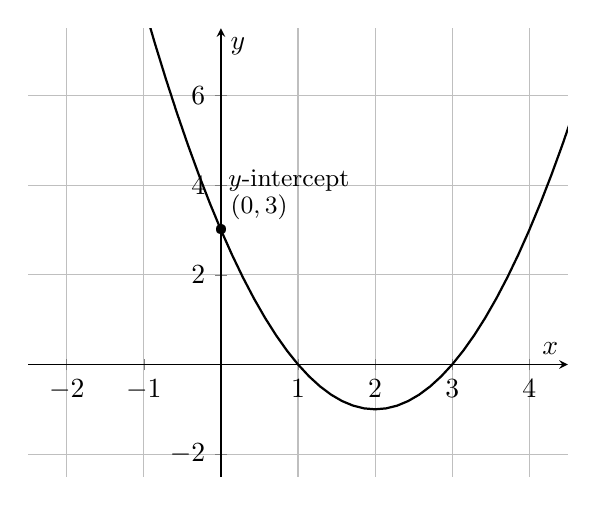
\begin{tikzpicture}
\begin{axis}[
    axis x line=center,
    xlabel={$x$},
    axis y line=center,
    ylabel={$y$},
    xmin=-2.5,
    xmax=4.5,
    ymin=-2.5,
    ymax=7.5,
    grid,
    % ytick={-1,...,8},
]
\addplot[domain=-2:5,samples=50,mark=none,thick]{x^2-4*x+3};
% \node [right] at (axis cs: 4.5,0) {$x$};
% \node [above] at (axis cs: -1,11) {$f(x)$};
\node at (axis cs: 0,3) {\textbullet};
\node (coord) [above right,font=\small] at (axis cs: 0,3) {$(0,3)$};
\node [above right=-2mm and -10mm of coord,font=\small]  {$y$-intercept};
% \node (zero0) at (axis cs: 1,0) {\textbullet};
% \node (zero1) at (axis cs: 3,0) {\textbullet};
% \node (label) at (axis cs: 1,2) {zeroes};
% \draw[very thick,->] (label.south) to (zero0.north east);
% \draw[very thick,->] (label.south) to (zero1.north west);
\end{axis}
\end{tikzpicture}
% \caption{The graph of the polynomial $f(x)=x^1-4x+3$ with the $y$-intercept labeled.}
\end{center}

You may have plotted polynomials before to show how the value of the polynomial changes 
with different values of $x$. A plot of our example polynomial is shown above.
In that case, we are plotting the equation 
\[
    f(x) = x^2 - 4x + 3
\]

where $f(x)$ is read as ``$f$ of $x$'' and indicates that the expression 
to the right of the equal sign is a function of the variable $x$. 
The \emph{$y$-intercept} of a function is the place it crosses the $y$-axis, 
i.e. its value when $x=0$. In our example, the $y$-intercept is 3. Notice 
that we could have calculated it without plotting the equation:
\[
    f(0) = (0)^2 - 4(0) + 3 = 3
\]



When a polynomial is written in standard form as in (\ref{eqn:std-form}), 
the $y$-intercept is $a_0$.

% The \emph{zeroes} of a function are the places where it crosses the $x$-axis,
% i.e. the values of $x$ for which $f(x)=0$. The zeroes in our example are 1 
% and 3:

% \begin{align*}
%     f(1) &= (1)^2 - 4(1) + 3 = 1 - 4 + 3 = 0\\
%     f(3) &= (3)^2 - 4(3) + 3 = 9 - 12 + 3 = 0
% \end{align*}

\begin{exercise}
    Write down the degree and $y$-intercept of each of the following 
    polynomials:
    \renewcommand{\labelenumi}{(\alph{enumi})} 
    \begin{enumerate}
        \item $f(x) = x^2 + 3x - 1$
        \item $f(x) = 5x^2 + 11$
        \item $f(x) = -2x^3 - x^2 + 9x$
        \item $f(x) = 3x^5 - 2x^3 - 15$
        \item $f(x) = (x^2-1)(x+3)$
        \item $f(x) = 2(x-6)(x+2)(x-5)$
        \item $f(x) = 2x^3(x+16)$
    \end{enumerate}
\end{exercise}

\subsubsection{Uniqueness}\label{sec:unique}

An important property of polynomials that they can be uniquely defined 
by a set of points of the right size. For example, two points uniquely 
define a line:

\begin{center}
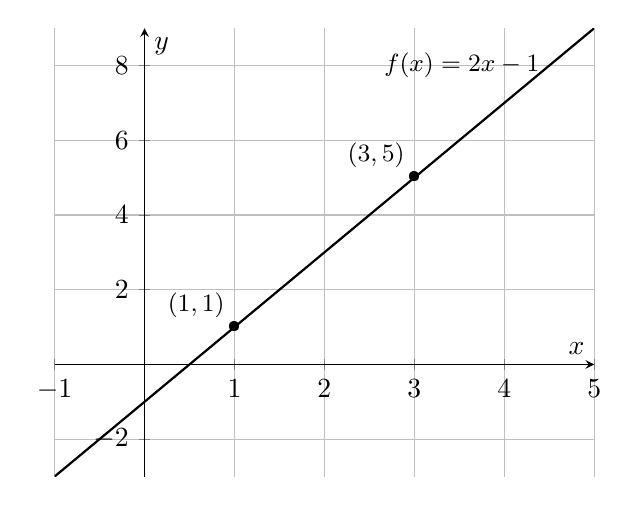
\begin{tikzpicture}
\begin{axis}[
    axis x line=center,
    xlabel={$x$},
    axis y line=center,
    ylabel={$y$},
    % xmin=-1.5,
    % xmax=5.5,
    % ymin=-1.5,
    % ymax=8.5,
    grid,
    % ytick={0,...,8},
]
\addplot[domain=-1:5,samples=50,mark=none,thick]{2*x-1};
\node (point1) at (axis cs: 1,1) {\textbullet};
\node [above left,font=\small] at (point1) {$(1,1)$};
\node (point2) at (axis cs: 3,5) {\textbullet};
\node [above left,font=\small] at (point2) {$(3,5)$};
\node [left,font=\small] at (axis cs: 4.5,8) {$f(x)=2x-1$};
\end{axis}
\end{tikzpicture}
\end{center}

Remember that a line can be viewed as a degree-1 polynomial! 
So, instead of giving someone the equation for this line, you could 
give them 2 points (for example, $(1,1)$ and $(3,5)$) and they'd 
still know exactly what line you're talking about. 

To specify a particular degree-2 polynomial, two points aren't enough.
For example, $x^2-4x+3$ goes through the points $(0,3)$ and $(4,3)$,
but so do many other degree-2 polynomials (represented here with dotted
lines):

\begin{center}
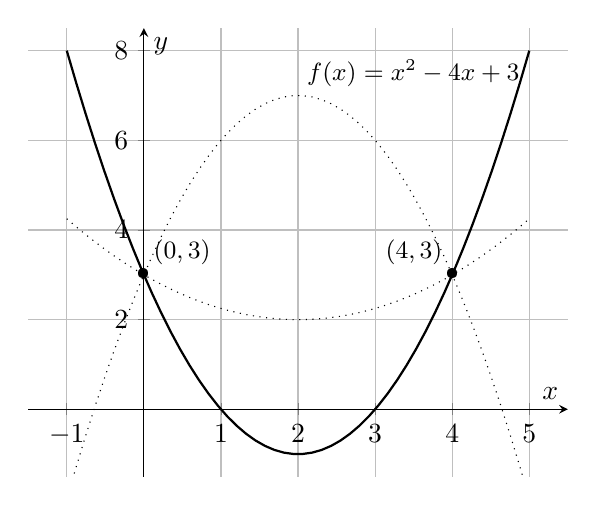
\begin{tikzpicture}
\begin{axis}[
    axis x line=center,
    xlabel={$x$},
    axis y line=center,
    ylabel={$y$},
    xmin=-1.5,
    xmax=5.5,
    ymin=-1.5,
    ymax=8.5,
    grid,
    % ytick={0,...,8},
]
\addplot[domain=-1:5,samples=50,mark=none,thick]{x^2-4*x+3};
\node (point1) at (axis cs: 0,3) {\textbullet};
\node [above right,font=\small] at (point1) {$(0,3)$};
\node (point2) at (axis cs: 4,3) {\textbullet};
\node [above left,font=\small] at (point2) {$(4,3)$};
\node [left,font=\small] at (axis cs: 5,7.5) {$f(x)=x^2-4x+3$};
% other degree-2 polys through these points
\addplot[domain=-1:5,samples=50,mark=none,dotted]{-(x^2-4*x+3)+6};
\addplot[domain=-1:5,samples=50,mark=none,dotted]{x^2/4-x+3};
\end{axis}
\end{tikzpicture}
\end{center}

Instead, 3 points are needed to uniquely define a degree-2 polynomial:

\begin{center}
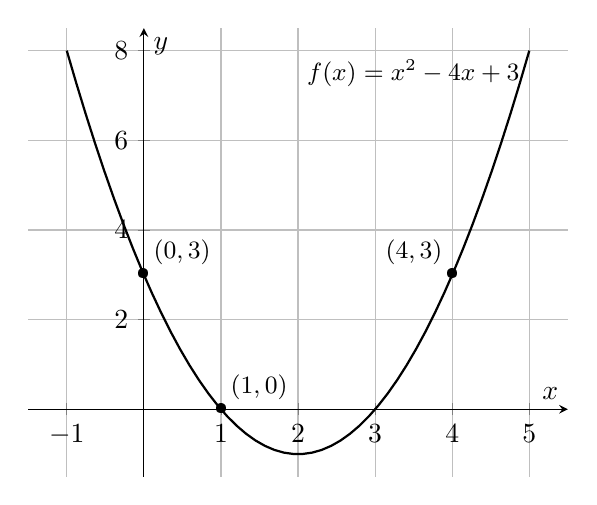
\begin{tikzpicture}
\begin{axis}[
    axis x line=center,
    xlabel={$x$},
    axis y line=center,
    ylabel={$y$},
    xmin=-1.5,
    xmax=5.5,
    ymin=-1.5,
    ymax=8.5,
    grid,
    % ytick={0,...,8},
]
\addplot[domain=-1:5,samples=50,mark=none,thick]{x^2-4*x+3};
\node (point1) at (axis cs: 0,3) {\textbullet};
\node [above right,font=\small] at (point1) {$(0,3)$};
\node (point2) at (axis cs: 4,3) {\textbullet};
\node [above left,font=\small] at (point2) {$(4,3)$};
\node (point3) at (axis cs: 1,0) {\textbullet};
\node [above right,font=\small] at (point3) {$(1,0)$};
\node [left,font=\small] at (axis cs: 5,7.5) {$f(x)=x^2-4x+3$};
\end{axis}
\end{tikzpicture}
\end{center}

How many points do you think are needed to uniquely define a degree-$n$
polynomial? Once you think you have an answer, flip to the next page.

\newpage
The process of recovering a polynomial passing through a set of points is 
called \emph{interpolation}. Accordingly, this general rule about the 
uniqueness of a polynomial described by a set of points is called the 
interpolation theorem:

\setlength\fboxsep{1em}        
\begin{center}
\fbox{
    \begin{minipage}{.7\linewidth}
        % \textbf{Interpolation Theorem.} \\
        \textsc{Interpolation Theorem.} \\
        Given a set of $t+1$ points, there 
        exists a unique degree-$t$ polynomial passing through those points.
    \end{minipage}
}
\end{center}

\begin{exercise}
    How many points are needed to uniquely define each polynomial 
    in the previous exercise?
\end{exercise}

If getting from a set of points to an equation sounds difficult, don't worry because 
there are well-known techniques that always work. Most programming languages 
actually have these built-in, so you don't need to know the details; you just 
plug points in and out comes a polynomial! In case you want to know more, though,
the next section explains how one of these techniques works.

\subsubsection{Lagrange Interpolation*}\label{sec:lagrange}

In this section we'll learn about one method of doing polynomial interpolation 
called \emph{Lagrange interpolation}. It's described by a single equation:

\begin{equation}\label{eqn:lagrange}
    P(x) = \sum_{i=0}^{n-1} y_i \ell_i(x), \text{ where } 
    \ell_i(x) = \prod_{\substack{j=0\\j\neq i}}^{n-1} \frac{x-x_j}{x_i-x_j}
\end{equation}

Let's break it down bit by bit. First, in case you aren't familiar with 
the symbols, $\sum_{i=0}^{n-1}$ \new{is called \emph{summation notation} 
or \emph{sigma notation}}. It means to evaluate the expression after 
$\sum$ for each value of $i$ \new{(starting at the number below the summation 
symbol and ending at the number above)} and then add all those terms together. For 
example:

\[
    \sum_{i=1}^n i = 1 + 2 + \ldots + n
\]

$\prod$ \new{(\emph{product notation} or \emph{pi notation})} is similar, but we multiply the expressions instead of adding 
them:
\[
    \prod_{i=1}^n i = 1 \cdot 2 \cdot \ldots \cdot n
\]

So, $\sum_{i=1}^{4} i = 1+2+3+4 = 10$ and $\prod_{i=1}^4 i = 1 \cdot 2 \cdot 3 
\cdot 4 = 24$.

\begin{bonus}
    Evaluate the following expressions:
    \renewcommand{\labelenumi}{(\alph{enumi})} 
    \begin{enumerate}
        \item $\sum_{i=1}^5 2i$
        \item $\sum_{i=1}^5 1$
        \item $\sum_{i=0}^4 x_i$ where $x_i$ means the $i$th 
        elements of the set $\{1, 5, -3, 0, 8\}$ and the numbering
        starts at 0 (that is, $x_0=1$).
        \item $\sum_{i=0}^2 x_i$ for the same set.
    \end{enumerate}
\end{bonus}

\begin{bonus}
    Repeat the previous exercise, substituting $\prod$ for $\sum$.
\end{bonus}

Now, back to Lagrange interpolation. We start with a set of points $(x_0, y_0), 
\ldots,\allowbreak (x_n, y_n)$. For each point $(x_i, y_i)$, we compute the 
expression $\ell_i(x)$. For instance, for $i=2$, it will be of the form

\newcommand{\cyan}[1]{\textcolor{cyan}{#1}}
\[
    \setlength{\fboxsep}{.3\fboxsep}
    \frac{x-\boxed{x_0}}{x_2-\boxed{x_0}}
    \frac{x-\boxed{x_1}}{x_2-\boxed{x_1}}
    \frac{x-\boxed{x_3}}{x_2-\boxed{x_3}}
    \cdots
    \frac{x-\boxed{x_n}}{x_2-\boxed{x_n}}
\]

Then we plug that expression $\ell_i(x)$, along with the $y$-value $y_i$ 
for that point, into the summation, and we'll end up with a polynomial. 
If we did everything right, that will be exactly the polynomial defined 
by those points.

Let's work through an example using the degree-1 polynomial from Section~\ref{sec:unique}:
we'll use the points $(1,1), (3,5)$ to recover the equation of the line. Remember that we 
start numbering the elements of a set at 0, so $(1,1)$ is the 0th point and $(3,5)$ is 
the 1st.

\begin{example}
Use Lagrange interpolation to get a degree-1 polynomial passing through the points 
$(1,1), (3,5)$.

Since we have $2$ points, $n=2$:
\begin{align*}
    P(x) &= \sum_{i=0}^{1} y_i \ell_i(x)\\
    &= y_0 \ell_0(x) + y_1 \ell_1(x)
\end{align*}

Next, let's substitute in the $y$-coordinates of our points:
\[
    = 1 \cdot \ell_0(x) + 5 \cdot \ell_1(x)
\]

Now let's evaluate the polynomials $\ell_i(x)$:

\begin{align*}
    \ell_0(x) &= \prod_{\substack{j=0\\j\neq 0}}^{1} \frac{x-x_j}{x_0-x_j}\\
    &= \frac{x-x_1}{x_0-x_1}\\
    &= \frac{x-3}{1-3}
    = \frac{x-3}{-2}\\
    \ell_1(x) &= \prod_{\substack{j=0\\j\neq 1}}^{1} \frac{x-x_j}{x_1-x_j}\\
    &= \frac{x-x_0}{x_1-x_0}\\
    &= \frac{x-1}{3-1}
    = \frac{x-1}{2}
    % \ell_i(x) &= \prod_{\substack{j=0\\j\neq i}}^{n-1} \frac{x-x_j}{x_i-x_j}
\end{align*}

Plugging that back into the sum, we get

\begin{align*}
    P(x) &= 1 \cdot \ell_0(x) + 5 \cdot \ell_1(x)\\
    &= 1 \left(\frac{x-3}{-2}\right) + 5 \left(\frac{x-1}{2}\right)\\
    &= \frac{-(x-3)}{2} + \frac{5(x-1)}{2}\\
    &= \frac{5x-5-(x-3)}{2}\\
    &= \frac{4x-2)}{2}
    = 2x-1\\
\end{align*}

That's the same equation as the one we graphed!
\end{example}

\begin{example}
Let's do the degree-2 example from Section~\ref{sec:unique} next. Our set of 
points is $\{(0,3),(1,0),(4,3)\}$ and $n=3$.
\begin{align*}
    P(x) &= \sum_{i=0}^{2} y_i \ell_i(x)\\
    &= y_0 \ell_0(x) + y_1 \ell_1(x) + y_2 \ell_2(x)\\
    &= 3 \cdot \ell_0(x) + 0 \cdot \ell_1(x) + 3 \cdot \ell_2(x)
\end{align*}

The polynomials $\ell_i(x)$ are:
\begin{align*}
    \ell_0(x) &= \prod_{\substack{j=0\\j\neq 0}}^{2} \frac{x-x_j}{x_0-x_j}\\
    &= \frac{x-x_1}{x_0-x_1} \frac{x-x_2}{x_0-x_2}\\
    &= \frac{x-1}{0-1} \frac{x-4}{0-4}\\
    &= \frac{x-1}{-1} \frac{x-4}{-4}
    = \frac{(x-1)(x-4)}{4}\\
    \ell_1(x) &= \prod_{\substack{j=0\\j\neq 1}}^{2} \frac{x-x_j}{x_1-x_j}\\
    &= \frac{x-x_0}{x_1-x_0} \frac{x-x_2}{x_1-x_2}\\
    &= \frac{x-0}{1-0} \frac{x-4}{1-4}\\
    &= \frac{x}{1} \frac{x-4}{-3}
    = \frac{x(x-4)}{-3}\\
    \ell_2(x) &= \prod_{\substack{j=0\\j\neq 2}}^{2} \frac{x-x_j}{x_2-x_j}\\
    &= \frac{x-x_0}{x_2-x_0} \frac{x-x_1}{x_2-x_1}\\
    &= \frac{x-0}{4-0} \frac{x-1}{4-1}\\
    &= \frac{x}{4} \frac{x-1}{3}
    = \frac{x(x-1)}{12}\\
    % \ell_i(x) &= \prod_{\substack{j=0\\j\neq i}}^{n-1} \frac{x-x_j}{x_i-x_j}
\end{align*}

Now we can simplify $P(x)$ to get:

\begin{align*}
    P(x) &= 3 \cdot \ell_0(x) + 0 \cdot \ell_1(x) + 3 \cdot \ell_2(x)\\
    &= 3 \cdot \frac{(x-1)(x-4)}{4} + 0 \cdot \frac{x(x-4)}{-3} + 3 \cdot \frac{x(x-1)}{12}\\
    &= \frac{3(x-1)(x-4)}{4} + \frac{3x(x-1)}{12}\\
    &= \frac{9(x-1)(x-4) + 3x(x-1)}{12}\\
    &= \frac{9(x^2-5x+4) + (3x^2-3x)}{12}\\
    &= \frac{9x^2-45x+36 + 3x^2-3x}{12}\\
    &= \frac{12x^2-48x+36}{12}\\
    &= x^2-4x+3
\end{align*}

and again we've arrived at the same polynomial we graphed.
\end{example}

\begin{bonus}
    Use Lagrange interpolation to find the unique degree-2 
    polynomial through the points $\{(-1,-16),(1,-2),(2,14)\}$.
\end{bonus}

\subsection{Sharing Secrets Using Polynomials}

Shamir secret sharing is a $(t+1)$-out-of-$n$ secret sharing scheme, for some numbers $t$ and $n$. This means that we split the secret $s$ into $n$ values and distribute them to $n$ people. Then, at least $t+1$ of those people must work together to recover $s$.

Let's update our definition of secret sharing from Section~\ref{sec:formal-defs}
to include $(t+1)$-out-of-$n$ secret sharing schemes where $t+1 \neq n$.

% This is the (t+1)-out-of-n definition
\begin{definition}[Secret sharing scheme (updated)]\label{def:ss-update}
    Let $\D$ be the input domain and $\D_s$ be the share domain.
    A secret sharing scheme is a pair of efficient algorithms $(\share, \rec)$
    and two associated natural numbers $t,n$ such that

    \begin{itemize}
        \item \share~takes as input a secret $s \in \D$ and outputs $n$ 
        shares in $\D_s$.
        \item \rec~takes as input $m$ shares $s_1, \ldots, s_m \in D_s$ 
        and output some value $y \in \D$ or a special symbol $\perp$ 
        indicating failure. (If $m < t+1$, it outputs $\perp$.)
    \end{itemize}
\end{definition}

Now we're ready to put everything we've learned together and define 
Shamir's secret sharing scheme\footnotemark.
\footnotetext{Adi Shamir introduced this scheme in a short 1979 
paper entitled ``How to share a secret''\cite{shamir1979share}.
The paper is only two pages long, so if you're feeling adventurous 
you could have a go at it! You can find it online at 
\url{http://web.mit.edu/6.857/OldStuff/Fall03/ref/Shamir-HowToShareASecret.pdf}.}

\begin{figure}[h!]
\begin{pchstack}[center]
\fbox{%
\procedure{$\share(s)$}{%
    a_1, \ldots, a_t \sample \{1, \ldots, 2^\lambda\} \\
    a_0 = s\\
    f(x) = a_t x^t + \ldots + a_1 x + a_0\\
    \pcreturn ((1,f(1)), \ldots, (n,f(n)))
}
\pchspace
\procedure[space=auto]{$\rec(s_1, \ldots, s_m)$}{%
    \pcif m < t+1 \pcthen\\
    \pcreturn \perp\\
    \pcelse\\
    f(x) = \textsf{interpolate}(s_1, \ldots, s_m)\\
    \pcreturn f(0)
}
}
\end{pchstack}
\caption{Shamir's secret sharing scheme}
\label{fig:shamirSS}
\end{figure}

To share a secret $s$ in $\D$, we choose a random 
degree-$t$ polynomial $f$ by sampling $t$ random coefficients and 
setting $f$'s $y$-intercept to the secret. Then we pick $n$ points 
on $f$ (the convention is to evaluate $f$ at 1, 2, and so on, up 
to $n$)\footnotemark. These $n$ points are the shares.
\footnotetext{To be exact, Shamir's secret sharing evaluates $f$ 
in a way that ensures the values $f(x_i)$ are elements of something 
called a \emph{finite field}. We won't go into details here about 
what that means, since such polynomials can't be graphed in two 
dimensions, but just know that this is important for the scheme 
to be truly private.}

To reconstruct, we need at least $t+1$ points. The reconstruction 
algorithm takes these points $s_i = (x_i, y_i)$ and tries to recover 
$f$ using interpolation. (If there are not enough points, interpolation 
would fail, so we return the symbol $\perp$ to indicate an error.)
Once we recover a polynomial, we evaluate it at 0 to find its 
$y$-intercept and output that.

\begin{example}
    Here's how we would compute $\share(12)$ with $t=1$ and $n=3$.
    First, we pick one random integer $a_1$, say $5$. Then $f(x)
    = 5x + 12$. Our three shares are $(1,17),(2,22),(3,27)$. Below 
    is a visual representation.
\end{example}

\begin{center}
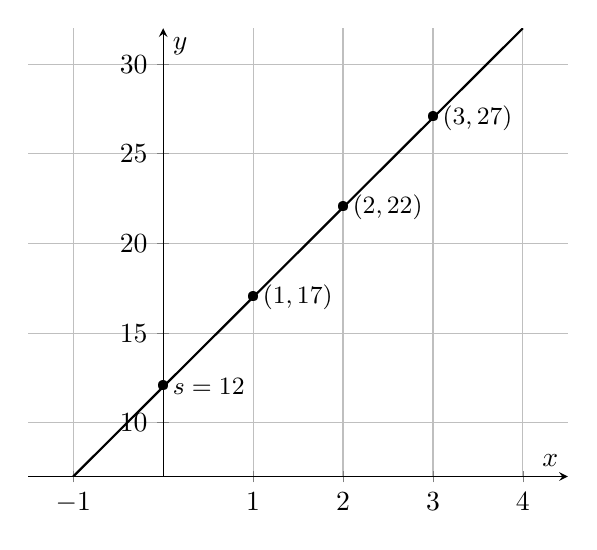
\begin{tikzpicture}
\begin{axis}[
    axis x line=center,
    xlabel={$x$},
    axis y line=center,
    ylabel={$y$},
    xmin=-1.5,
    xmax=4.5,
    % ymin=-2.5,
    % ymax=7.5,
    grid,
    % ytick={-1,...,8},
]
\addplot[domain=-1:4,samples=50,mark=none,thick]{5*x+12};
\node (share1) at (axis cs: 1,17) {\textbullet};
\node (share2) at (axis cs: 2,22) {\textbullet};
\node (share3) at (axis cs: 3,27) {\textbullet};
\node [right,font=\small] at (share1) {$(1,17)$};
\node [right,font=\small] at (share2) {$(2,22)$};
\node [right,font=\small] at (share3) {$(3,27)$};
\node (s) at (axis cs: 0,12) {\textbullet};
\node [right,font=\small] at (s) {$s=12$};
\end{axis}
\end{tikzpicture}
\end{center}

\begin{example}
    Now let's say we receive two of the previous shares to reconstruct:
    $(1,17),(3,27)$ We know they are 2-out-of-3 shares (this is realistic; 
    in practice, $t$ and $n$ would be known to all the parties, or the 
    points would be labeled with the values of $t$ and $n$ used to 
    generate them.) How do we reconstruct?

    First of all, \new{we know that reconstruction is possible} because 
    $t+1 = 2$ and we have at least two shares (exactly two, in fact). 
    \nsm{Is this wording less confusing?}
    Now we need to interpolate to recover the degree-2 polynomial 
    they represent. (If you didn't read Section~\ref{sec:lagrange}, 
    you can skip to the evaluation of $f(0)$ on the next page.)

    Let's re-number the input shares starting with 
    0, so $(x_0,y_0) = (1,17)$ and $(x_1,y_1) = (3,27)$.
    \begin{align*}
        f(x) &= \sum_{i=0}^{m} y_i \ell_i(x)\\
        &= y_0 \ell_0(x) + y_1 \ell_1(x)\\
        &= 17 \ell_0(x) + 27 \ell_1(x)
    \end{align*}

    At this point, we can take a little shortcut. We know we only 
    care about finding the value of $f$ at 0, which means we only 
    need to find $\ell_0(0)$ and $\ell_1(0)$ instead of the full 
    expressions. So,
    \begin{align*}
        \ell_0(0) &= \prod_{\substack{j=0\\j\neq 0}}^{1} \frac{0-x_j}{x_0-x_j}
        = \frac{-3}{1-3}
        = \frac{3}{2}\\
        \ell_1(0) &= \prod_{\substack{j=0\\j\neq 1}}^{1} \frac{0-x_j}{x_1-x_j}
        = \frac{-1}{3-1}
        = -\frac{1}{2}
    \end{align*}

    % \begin{align*}
    %     f(x) &= 17 \ell_0(x) + 27 \ell_1(x)\\
    %     f(x) &= 17 \frac{x-2}{-1} + 27 \frac{x-1}{1}\\
    %     f(x) &= -17(x-2) + 27(x-1)\\
    %     f(x) &= -10x+7
    % \end{align*}
    Then 
    \begin{align*}
        f(0) &= 17 \ell_0(0) + 27 \ell_1(0)\\
        &= 17 \cdot \frac{3}{2} + 27 \cdot -\frac{1}{2}\\
        &= \frac{51-27}{2}\\
        &= \frac{24}{2} = 12\\
    \end{align*}
\end{example}

\begin{bonus}\label{bon:rec-groups}
    Work in a small group. Everyone in the group should pick 
    a secret number to share. Let $n$ be the number of people in 
    your group and pick $t$ so that $t+1 < n$. Use \share~to 
    compute shares of your secret and give each person in the group
    one share. Now a subgroup of $t+1$ people should work together 
    to reconstruct the secret using \rec. Once they succeed, 
    form a different group of $t+1$ people and run \rec~again
    using this new group of points. You should get the same 
    result!
\end{bonus}

Notice that in the scheme presented in Figure~\ref{fig:shamirSS},
it's possible for someone to lie about their point, thereby 
causing the interpolation algorithm to return a different 
polynomial besides $f$. In that case, $f(0)$ might not equal $s$ 
and we'd recover the wrong secret!

This doesn't violate correctness, however, because in that case 
we aren't running \rec~on outputs of the \share~algorithm, so 
the correctness definition doesn't apply. Instead, what's happening 
is that our scheme fails when the parties don't behave honestly.
In cryptography, this means that the scheme is only secure in the 
presence of \emph{semi-honest} adversaries (the scheme has 
\emph{semihonest security}.) There are ways of fixing this scheme 
to guarantee security against \emph{malicious} adversaries 
(\emph{malicious security}), but that's outside the scope of this 
packet.

\begin{exercise}
    Visit \url{https://bit.ly/ShamirSS} in your browser. This is a 
    Google Colab notebook written in the Python programming language. 
    It already has the functions \share~and \rec~from Shamir's secret 
    sharing scheme. Work through the examples in the notebook to 
    share and reconstruct any numbers you want using this scheme, 
    then read on to find out how to share secret messages!
\end{exercise}

% TODO: if we use this exercise, must explain why $f$ needs to 
% be evaluated over a finite field
% \begin{bonus}
%     Show that Shamir secret sharing is private. (You can refer back to Section~\ref{sec:proof}
%     if necessary.)
% \end{bonus}

\section{Beyond secret sharing}

\new{Congratulations on making it through this packet! You have not only 
learned about secret sharing, a building block for many other cryptographic 
primitives that are used in the real world\footnotemark, but have also
gotten a glimpse into what modern cryptography research looks like. 
The same definitions and proof techniques you saw in this packet pop 
up in many other areas of cryptography, and you now have a head start in 
understanding the techniques in many other subfields.}

\footnotetext{\new{Most notably, secret sharing forms the basis of many 
\emph{multiparty computation (MPC)} schemes. These allow multiple 
parties, as the name implies, to compute functions over their secret 
inputs. For example, the Boston Women’s Workforce Council organized 
an effort which used MPC\cite[page 12]{bwwc} to calculate statistics 
about the salaries of the workforce in about 16\% of the Boston area to 
show that the gender pay gap was wider than what the U.S. Bureau of Labor
Statistics reported\cite{bwwc}. MPC was necessary because companies needed 
to keep their data on employee salaries secret due to privacy concerns.}}

\newpage
{\small
\bibliographystyle{unsrt}
\bibliography{main}
}
\end{document}
